\twocolumn[\colorsection{Calorimetría}]
\setcounter{figure}{0}
% %
% \begin{Exercise}
%   \textit{a}) La temperatura corporal normal promedio medida en la boca es $\SI{310}{\kelvin}$. ¿Cuál es la temperatura en grados Celsius y en Fahrenheit? \textit{b}) Durante un ejercicio muy vigoroso, la temperatura del cuerpo puede elevarse hasta $\SI{40}{\celsius}$. ¿Cuál es la temperatura en Kelvin y en grados Fahrenheit? \textit{c}) La temperatura de la superficie del cuerpo es aproximadamente $\SI{7}{\celsius}$ más baja que la temperatura interna. Exprese esta diferencia de temperatura en Kelvin y en grados Fahrenheit. \textit{d}) La sangre almacenada a $\SI{4}{\celsius}$ dura aproximadamente 3 semanas, mientras que la sangre almacenada a $\SI{-160}{\celsius}$ tiene una duración de 5 años. Exprese ambas temperaturas en las escalas Fahrenheit y Kelvin.
% \end{Exercise}
% \begin{Answer}
% 	\begin{minipage}[t]{.4\textwidth}
%     \textit{a}) $\SI{36.9}{\celsius}$ y $\SI{98.4}{^\circ F}$\\ \textit{b}) $\SI{313}{\kelvin}$ y $\SI{104}{^\circ F}$\\ \textit{c}) $\SI{7}{\kelvin}$ y $\SI{13}{^\circ F}$\\ \textit{d}) $\SI{4}{\celsius}$: $\SI{277}{\kelvin}$ y $\SI{39.2}{^\circ F}$; $\SI{-160}{\celsius}$: $\SI{113}{\kelvin}$ y $\SI{-256}{^\circ F}$
%   \end{minipage}
% \end{Answer}
%
\begin{Exercise}
  \textit{a}) Calcule la única temperatura a la que los termómetros Fahrenheit y Celsius coinciden. \textit{b}) Calcule la única temperatura a la que los termómetros Fahrenheit y Kelvin coinciden.
\end{Exercise}
\begin{Answer}
	\begin{minipage}[t]{.4\textwidth}
    \textit{a}) $\SI{-40}{\celsius}=\SI{-40}{^\circ F}$\\ \textit{b}) $\SI{575}{^\circ F}=\SI{575}{\kelvin}$
  \end{minipage}
\end{Answer}
%
\begin{Exercise}
  \textit{a}) Un termómetro de gas a volumen constante tiene una presión de $\SI{1000}{\pascal}$ a $\SI{15}{\celsius}$. Si la presión se incrementa a $\SI{2000}{\pascal}$, ¿cuál es la temperatura en grados Celsius? \textit{b}) Un termómetro de gas registra una presión absoluta de $\SI{325}{mmHg}$, estando en contacto con agua en el punto triple. ¿Qué presión indicará en contacto con agua en su punto de ebullición normal?
\end{Exercise}
\begin{Answer}
	\begin{minipage}[t]{.4\textwidth}
    \textit{a}) $\SI{303}{\celsius}$\\ \textit{b}) $\SI{444}{mmHg}$
  \end{minipage}
\end{Answer}
%
\begin{Exercise}
  Usando un termómetro de gas de volumen constante, un experimentador determinó que la presión del gas cuando el termómetro se encuentra a la temperatura del punto triple del agua ($\SI{0.01}{\celsius}$) es $\SI{4.8E4}{\pascal}$; y en el  punto de ebullición normal del agua ($\SI{100}{\celsius}$) es $\SI{6.5E4}{\pascal}$. \textit{a}) Suponiendo que la presión varía linealmente con la temperatura, use estos datos para calcular la temperatura Celsius en la que la presión del gas sería cero (es decir, obtenga la temperatura Celsius del cero absoluto). \textit{b}) ¿El gas de este termómetro obedece con precisión la ecuación $T_2/T_1=p_2/p_1$? Si es así y la presión a $\SI{100}{\celsius}$ fuera $\SI{6.5E4}{\pascal}$, ¿qué presión habría medido el experimentador a $\SI{0.01}{\celsius}$?
\end{Exercise}
\begin{Answer}
	\begin{minipage}[t]{.4\textwidth}
    \textit{a}) $\SI{-282.4}{\celsius}$\\ \textit{b}) $\SI{4.6E4}{\pascal}$
  \end{minipage}
\end{Answer}
%
\begin{Exercise}\label{p:calorimetria01}
  Un técnico mide el calor específico de un líquido desconocido sumergiendo en él una resistencia eléctrica. La energía eléctrica se convierte en calor transferido al líquido durante $\SI{120}{\second}$ a una tasa constante de $\SI{65.0}{\watt}$. La masa del líquido es $\SI{0.780}{\kilogram}$ y su temperatura aumenta de $\SI{18.55}{\celsius}$ a $\SI{22.54}{\celsius}$. Calcule el calor específico promedio del líquido en este intervalo de temperatura. Suponga que la cantidad de calor que se transfiere al recipiente es despreciable y que no se transfiere calor al entorno.
\end{Exercise}
\begin{Answer}
  $\SI{2.51E3}{\joule.\kilogram^{-1}.\kelvin^{-1}}$
\end{Answer}
%
\begin{Exercise}\label{p:calorimetria02}
  \ifthenelse{\equal{\seleccionados}{true}}
    {\addToList{xyz-calorimetria}{\ExerciseHeaderNB}}{}
  En un experimento se suministra calor a una muestra sólida de $\SI{500}{g}$ a una tasa de $\SI{10.0}{\kilo\joule/\minute}$ mientras se registra su temperatura en función del tiempo. La gráfica de sus datos se muestra en la figura \ref{f:calorimetria02}. \textit{a}) Calcule el calor latente de fusión del sólido. \textit{b}) Determine los calores específicos de los estados sólido y líquido del material.
\end{Exercise}
\begin{Answer}
	\begin{minipage}[t]{.4\textwidth}
    \textit{a}) $ L_f = \SI{3.00E4}{\joule/\kilogram}$\\ \textit{b}) $c_\text{sólido}=\SI{1.33E3}{\joule.\kilogram^{-1}.\kelvin^{-1}}$ y $c_\text{líquido}=\SI{1.00E3}{\joule.\kilogram^{-1}.\kelvin^{-1}}$
  \end{minipage}
\end{Answer}
%
\begin{center}
  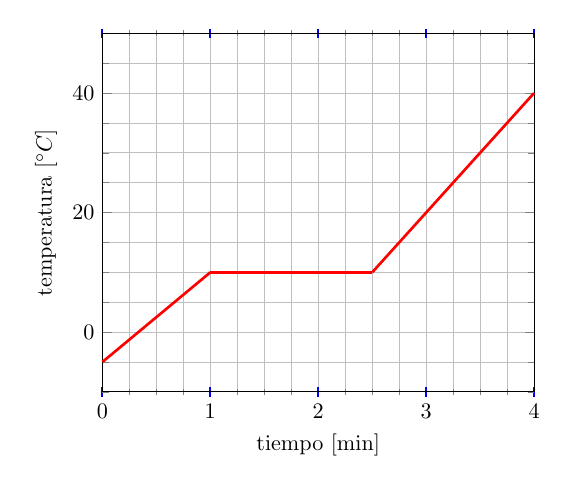
\begin{tikzpicture}[scale=0.8]
      \begin{axis}[
                   every major x tick/.append style={thick,blue},
                   clip=false,
                   grid=both,
                   minor x tick num=3,        %un minor tick es decir 0.5
                   minor y tick num=3,
                   xmin=0, xmax=4,           %min y max para los ejes, NO PARA EL DOMINIO
                   ymin=-10, ymax=50,
                   %axis y line=center,        %alinea el eje al centro de la figura
                   %axis x line=middle,        %sino pone 2 ejes x
                   xtick  align=center,
                   xlabel={tiempo~[min]},
                   ylabel={temperatura~[$^\circ\text{C}$]}
                  ];
      \addplot [color=red, very thick] [id=s,samples= 180, domain=0:1]  {-5+15*x};
      \addplot [color=red, very thick] [id=s,samples= 180, domain=1:2.5]  {10};
      \addplot [color=red, very thick] [id=s,samples= 180, domain=2.5:4]  {10+20*(x-2.5)};
      \end{axis}
    \end{tikzpicture}
    \captionof{figure}{Problema \ref{p:calorimetria02}\label{f:calorimetria02}}
  \end{center}
%
\begin{Exercise}
  \ifthenelse{\equal{\seleccionados}{true}}
    {\addToList{xyz-calorimetria}{\ExerciseHeaderNB}}{}
  Una pieza metálica de $\SI{6.00}{\kilogram}$ de cobre sólido a una temperatura inicial $T$ se coloca con $\SI{2.00}{\kilogram}$ de hielo que se encuentran inicialmente a $\SI{-20.0}{\celsius}$. El hielo está en un contenedor aislado de masa despreciable. Después de que se alcanza el equilibrio térmico, se observan $\SI{1.20}{\kilogram}$ de hielo y $\SI{0.80}{\kilogram}$ de agua líquida. ¿Cuál era la temperatura inicial de la pieza de cobre?
\end{Exercise}
\begin{Answer}
  $T=\SI{150}{\celsius}$
\end{Answer}
%
\begin{Exercise}
  \ifthenelse{\equal{\seleccionados}{true}}
  {\addToList{xyz-calorimetria}{\ExerciseHeaderNB}}{}
  Una olla de cobre con una masa de $\SI{0.500}{\kilogram}$ contiene $\SI{0.170}{\kilogram}$ de agua, y ambas están a una temperatura de $\SI{20.0}{\celsius}$. Un bloque de $\SI{0.250}{\kilogram}$ de hierro a $\SI{85.0}{\celsius}$ se deja caer en la olla. Encuentre la temperatura final del sistema, suponiendo que no hay pérdida de calor a los alrededores.
\end{Exercise}
\begin{Answer}
  $\SI{27.5}{\celsius}$
\end{Answer}
%
\begin{Exercise}
  En un recipiente adiabático de masa despreciable, $\SI{0.2}{\kilogram}$ de hielo a una temperatura inicial de $\SI{-40}{\celsius}$ se mezclan con una masa $m$ de agua que tiene una temperatura inicial de $\SI{80}{\celsius}$. Si la temperatura final del sistema es $\SI{20}{\celsius}$, ¿cuál es la masa $m$ del agua que estaba inicialmente a $\SI{80}{\celsius}$?
\end{Exercise}
\begin{Answer}
  $m=\SI{0.4}{\kilogram}$
\end{Answer}
%
\begin{Exercise}
  El calor específico molar de cierta sustancia varía con la temperatura según la siguiente ecuación empírica: $C = a + bT$, donde $a=\SI{29.5}{\joule.\mole^{-1}.\kelvin^{-1}}$ y $b=\SI{8.20E-3}{\joule.\mole^{-1}.\kelvin^{-2}}$. ¿Cuánto calor se necesita para modificar la temperatura de $\SI{3.00}{\mole}$ de la sustancia de $\SI{27.0}{\celsius}$ a $\SI{227}{\celsius}$? (Sugerencia: Integre la ecuación $dQ = nCdT$.)
\end{Exercise}
\begin{Answer}
  $Q=\SI{19700}{\joule}$
\end{Answer}
%
\begin{Exercise}
  Un calorímetro de cobre cuya masa es $\SI{0.446}{\kilogram}$ contiene $\SI{0.095}{\kilogram}$ de hielo, y el sistema está inicialmente en equilibrio a $\SI{0}{\celsius}$. Si se agregan $\SI{0.035}{\kilogram}$ de vapor de agua a $\SI{100.0}{\celsius}$ y $\SI{1}{atm}$ de presión, \textit{a}) ¿qué temperatura final alcanzará el calorímetro y su contenido?, \textit{b}) ¿cuántos kilogramos habrá de hielo, de agua líquida y de vapor a dicha temperatura final?
\end{Exercise}
\begin{Answer}
	\begin{minipage}[t]{.4\textwidth}
    \textit{a}) $\SI{86.2}{\celsius}$\\ \textit{b}) sin hielo, sin vapor, $\SI{0.130}{\kilogram}$ de agua en estado líquido.
  \end{minipage}
\end{Answer}
%
\begin{Exercise}
  Un calorímetro cuyo equivalente en agua es $\SI{20}{\gram}$, contiene $\SI{100}{\gram}$ de agua a $\SI{20}{\celsius}$. Se agregan $\SI{50}{\gram}$ de una sustancia desconocida a una temperatura de $\SI{90}{\celsius}$, obteniéndose una temperatura final de equilibrio de $\SI{24}{\celsius}$. Calcular el calor específico de la sustancia desconocida.
\end{Exercise}
\begin{Answer}
  $\SI{0.145}{cal.\gram^{-1}.\celsius^{-1}}$
\end{Answer}
%
\begin{Exercise}
  \ifthenelse{\equal{\seleccionados}{true}}
  {\addToList{xyz-calorimetria}{\ExerciseHeaderNB}}{}
  Un calorímetro contiene $\SI{40}{\gram}$ de agua a $\SI{22}{\celsius}$ y se le agregan $\SI{50}{\gram}$ de agua a $\SI{50}{\celsius}$, obteniéndose una temperatura final de $\SI{35}{\celsius}$. \textit{a}) Calcular el equivalente en agua del calorímetro. \textit{b}) En un nuevo experimento, este mismo calorímetro contiene $\SI{100}{\gram}$ de agua a una temperatura de $\SI{22}{\celsius}$, y se agregan $\SI{80}{\gram}$ de aluminio a $\SI{90}{\celsius}$. Calcular la temperatura de equilibrio. \textit{Dato:} Calor específico del aluminio: $\SI{0.22}{cal.\gram^{-1}.\celsius^{-1}}$.
\end{Exercise}
\begin{Answer}
	\begin{minipage}[t]{.4\textwidth}
    \textit{a}) $\SI{17.7}{\gram}$\\ \textit{b}) $\SI{30.8}{\celsius}$
  \end{minipage}
\end{Answer}
%
